\documentclass[a4paper,12pt]{article}
\usepackage[utf8]{inputenc}
\usepackage{graphicx}
\usepackage{float}

%opening
\title{TOK: Are some things unknowable?}
\author{Terry Qi}

\begin{document}

\maketitle
\begin{enumerate}
 \item Law of demand
 \item Double Pendulum
 \item Progress bars
\end{enumerate}

\begin{figure}[h!]
 \centering
 \[
    Q = a - bP
 \]
 \caption{The law of demand}
\end{figure}

\begin{figure}[h!]
 \centering
 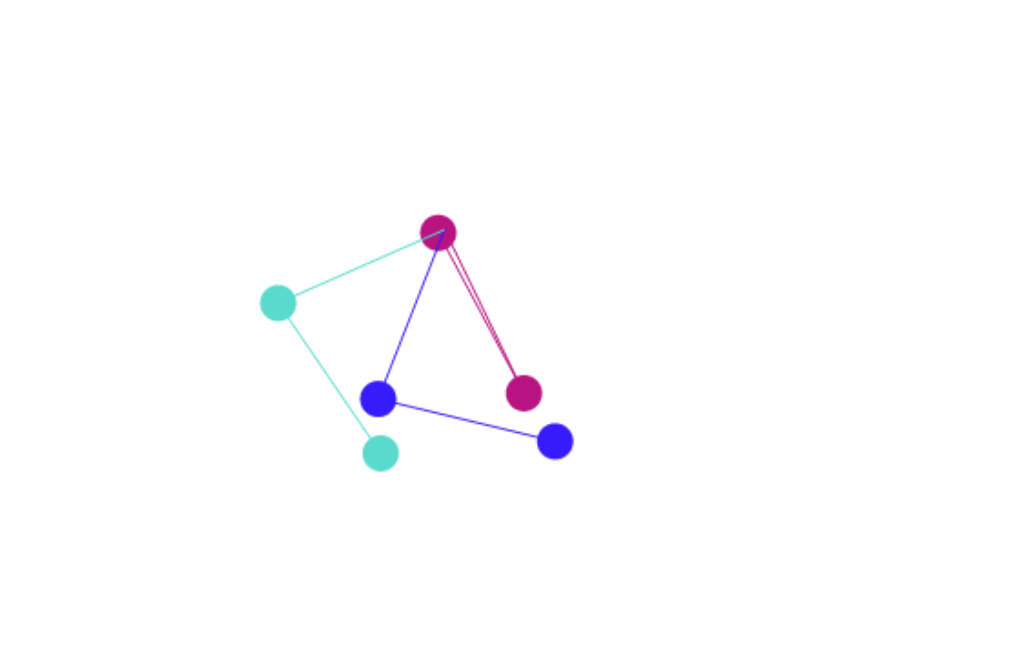
\includegraphics[scale=0.25]{dpend.png}
 \caption{Three Double Pendulums}
\end{figure}

\begin{figure}[h!]
 \centering
 
\includegraphics[scale=0.35]{progress.png}
 \caption{A progress bar}
\end{figure}



\newpage

% breakdown of 
% theme of does empirical evidence impiy knowledge in the sciences. question
% LOD: social sciences, hypothesize, trend
% double pendulum: the natural sciences, chaotic application, predicable path, yet no knowledge of its location
% progress bar: provenable knowable yet pretend to be in control. questions the motivation to certainty, 


% intro
The TOK prompt I have chosen is: ``Are some things unknowable?''. This exhibition will explore the prompt by reflecting upon knowledge and sciences, more specifically answering whether empirical evidence hinder in the acceptance of knowledge in the sciences. While in the area of Mathematics we often take deductive reasoning as granted, this is less common in 


% knowable thing but could be failified
\paragraph{1}

% knowable thing but is chaotic
\paragraph{2}

% unknowable thing that expresses certainty
\paragraph{3}

\end{document}
